\chapter{Identification in Diabetes}
\label{sec:IdentificationInDiabetes}

%Incluir detalles de estudios realizados con datos en diabetes. Stahl, tesina, palerm, finan, etc

Insulin treatment is currently a necessity for T1DM patients. The insulin dose must be individualized foreach patient and for that physicians have traditionally characterized the patients using clinical parameters tuned heuristically. Such parameters represent an estimation of the insulin effect on glucose metabolism and the quality of glucose control depends on the performance of the parameters estimation. The latter is time consuming and requires constant patient reevaluation by a skilled health-care team. As a common consequence there is a mismatch between patient's needs and the actual insulin treatment, resulting in suboptimal glycaemic control.

In the artificial pancreas context the characterization of a patient is required to be much more accurate. Model individualization is required for every patient in order to get accurate enough predictions of the blood glucose levels. Using mathematical models for glucose prediction has been present in diabetes literature since the first models were published, but few satisfying results have been achieved for long term predictions. 

Patient identification deals with inter-patient (between patients) variability. The problem of characterizing inter-patient variability is handled individualizing models for each patient independelty. Intra-patient variability is much difficult to quantify, and in this thesis it is the main problem to overcome by the methodology and experimentation here described. From this point onward when referring to variability only intra-patient (within the patient) variability will be accounted. Intra-patient variability is the compound effect of several factors: not measured methabolism, stress intensity, hour of the day and meal uncertainty among others. The effects of this variability can be observed in many of the measured and identified parameters, often resulting in poor repeatibility in parameter identification.

In this chapter the most important and latest findings published in literature related to model individualization for diabetes will be reviewed.

\section{Patient Identification}
\label{sec:GlucoseCurveFitting} 

Glucose prediction from identification of models using experimental glucose data can be classified according to the nature of the model used. As described in the models in Section \ref{sec:ModelsForDiabetes}, models for diabetes can be data-driven or physiology-driven. 

From the engineering point of view, St{\aa}hl and Johansson published a pilot identification study \cite{stahl2009diabetes} using modified models from literature and data-driven models. This paper describes the experience of the first author, whom was diagnosed with diabetes shortly before the study, analyzing and modeling his own glucose profile over a period of several weeks. They analyzed in detail the characteristics of the data-set, including auto-correlation function, probabilistic distribution of the samples, sampling times, and statistical properties. They used models in literature for the input models, using in both cases (insulin and meal) two different pathways for fast and slow inputs. As for the endogenous models, they tested a battery of grey-box, data-driven models, including Auto Regressive models with exogenous inputs (ARX), Auto Regressive Moving Average models with exogenous inputs (ARMAX), General Transfer Function Models (GTFM), and state space models of increasing complexity. They used the models for validation of the identified patient under different prediction horizons. The study concluded that GTFM were well suited for prediction up to 2 hours ahead (8 simulation steps), but further horizons of prediction were not possible using any of the models used. 
%\begin{figure}[hbt]
%\centering
%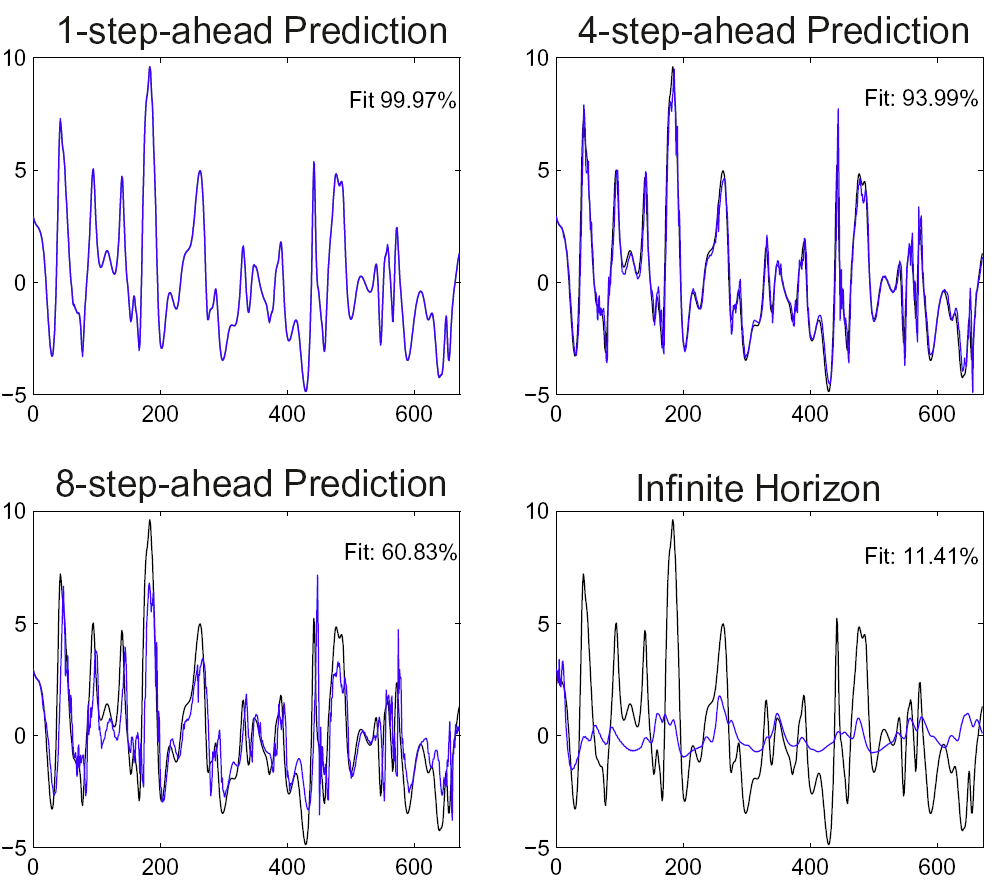
\epsfig{file=Figures/stahl.png, width=0.8\textwidth}\caption{Illustration of the degradation of predictive ability with the prediction horizon: upper left $\tau$ =1 (15 minutes); upper right $\tau$ =4 (1 hour); lower left $\tau$ =8 (2 hours); lower right $\tau =\infty$. Experimental data is plotted in black, and the predictions in blue.}
%\label{fig:stahl_compare}
%\end{figure}
The study performed by St{\aa}hl and Johansson was very useful in the diabetes identification scene as a pilot study, but it was nonetheless limited in many aspects. The data-set used was comprised only of data from one patient, thus neglecting completely the population variation in the diabetes metabolism. The study also only used self-measured capillary samples with irregular sampling times. Capillary blood glucose estimation can be subject to many errors and disturbances, and it is also too sparse to be able to capture glucose dynamics. More frequent sampling and more reliable measurements can improve the outcome of the study.

Johansson and his colleagues in Lund continued the investigation further on, publishing another study \cite{cescon2009subspace} where the effect of subspaced based models was considered. In this case, the data was taken from a patient that was wearing a CGM, monitored during three days under CSII (Continuous Subcutaneous Insulin Infusion) therapy, which provided with much more frequent data than in the previous study. Again, the models used for the inputs of the system where rather complex physiology-based models, like the UVA group meal model and the Cambridge insulin model described in chapters \ref{sec:ModelBasedOnDallaManEtAl} and \ref{sec:WillinskaEtAl} respectively. The rational behind this decision lies in the fact that the perturbations of the system (i.e. meals and insulin treatment) have an enormous impact on the diabetic patient glucose. The lack of physiologic insulin secretion in response to a meal make glucose homeostasis a hard task. In this context, insulin replacement in the subcutaneous tissue and meals represent a perturbation of the glucose system that needs a detailed description of the models used. This work showed that predictions with horizons larger than 30 minutes were very imprecise for CGM measurements. CGM involves more frequent sampling, but it introduces large errors in the measured blood glucose concentration, leading to great difficulties in the predictions. Nevertheless, this study introduces separation between meals and its related insulin dose and viceversa for easier identification, which is a concept that will be investigated later in this thesis.

Rollins \textit{et al.} published another self study, where a type 2 diabetic patient (Rollins himself) was monitored for several weeks \cite{rollins2010free} without insulin treatment. This study focused on predicting glucose by using many different measurements of the patients metabolism. The patient followed a normal life routine, wearing sensors of temperature, body activity, heat flux and CGM, as well as a diary with all relevant information about meals. They used data-driven models with multiple inputs in order to fit the patient's data. Model validation was performed against CGM estimations.
%\begin{figure}[hbtp]
%\centering
%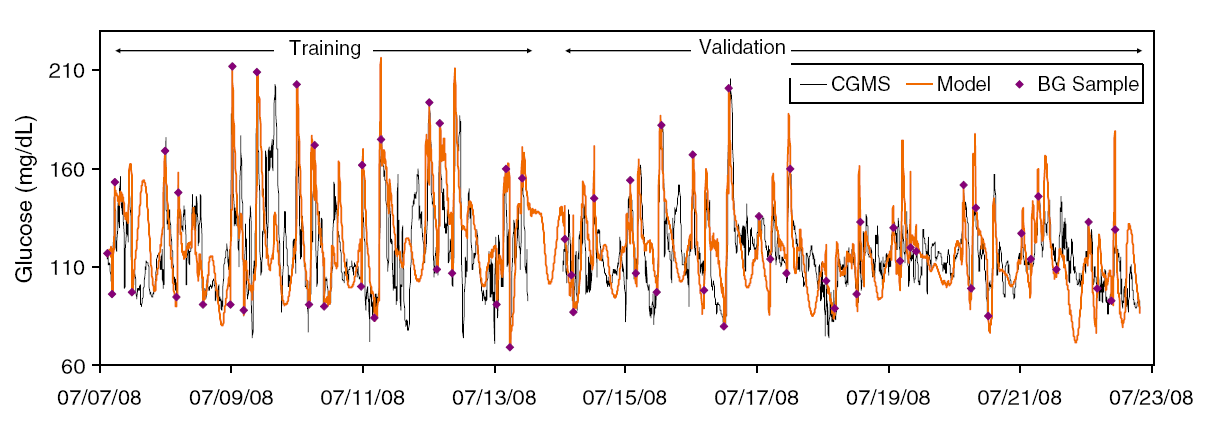
\epsfig{file=Figures/rollinsval.png, width=\textwidth}\caption{Model data fitting and validation of one of the models tested. Seven days were used for data fitting and 9 days for validation.}
%\label{fig:rollinsval}
%\end{figure}
Rollins showed that very good predictions ($r_{fit}$ up to 0.70) can be achieved if more data from the patient's metabolism and daily rhythm was provided. Unfortunately, these results are not extendable to type 1 diabetic patients since insulin treatments induce enormous perturbations to the system that were not modeled in this paper. Also, only 1 patient was monitored for this study, and diabetic patients may be reluctant to wear all the devices needed for full metabolic monitoring required for this study. Furthermore, complexity of this kind of monitoring make it unfeasible in clinical practice.

Georga \textit{et al.} studied the possibility of using a combination of physiological models as inputs to the system, and vector machine for regression as predictor of blood glucose \cite{georga2011glucose}. Their study comprised seven patients with 10 days average monitoring period. They incorporated the possibility of using an exercise model as an input to the glucose predictor. They showed results similar to those of \cite{rollins2010free}, but slightly less accurate predictions to those in \cite{stahl2009diabetes}, but comparisons between these studies are loosely sustained since the two previous studies only simulate one patient. No significant improvement was observed when including the exercise model into the prediction method.

In the work of Cameron \textit{et al.} on prediction of blood glucose for MPC controllers, a comparison of multiple models is performed \cite{cameron2012extended}. Four variations of a very simple data-driven model are tested for their predictive capabilities. The variations affect the meal prediction of the model in different ways, with increasing complexity:
\begin{itemize}
	\item No meal detection. Meals occur without announcement or reaction of the predictive model.
	\item Meal detection. Probabilistic detection of meals is implemented in the prediction model.
	\item Meal detection and anticipation. Meals are predicted and action is anticipated to the actual meal effect on glucose.
	\item Meal announcement. Meal time is assumed to be input by the user.
\end{itemize}
Prediction horizons of up to 5 hours are tested for all the variations of the model, both on simulated meal data and 19 days of experimental clinical data. Prediction capabilities are computed with mean error and root mean squared error (RMSE). Predictions are evaluated against prediction horizon on experimental data, and against time for a 2-hour prediction horizon in simulated meal data. This study presents large prediction errors (100 mg/dL) even for relatively short prediction horizon, but prediction performance increases as more information is estimated or provided to the model, being the meal announcement variation the most successful in terms of prediction capabilities.
%\begin{figure}[htb]
%\centering
%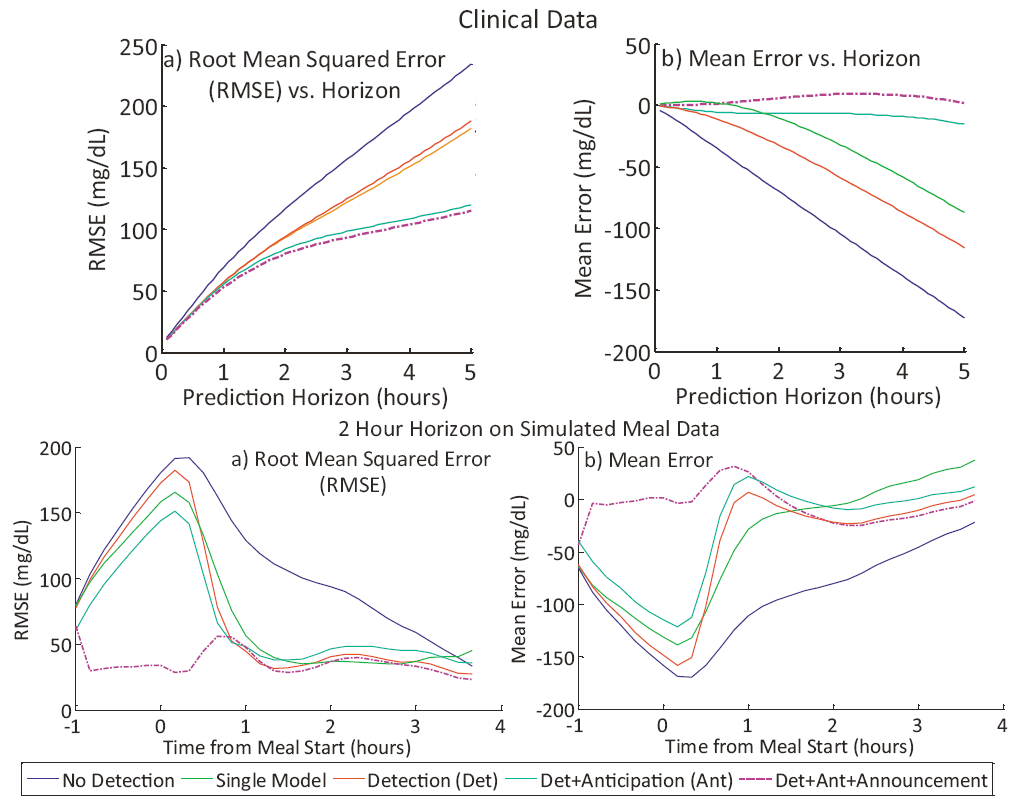
\epsfig{file=Figures/cameron_prediction.png, width=0.9\textwidth}\caption{Prediction results for all the variations of the model tested by Cameron \textit{et al.} Top panel presents the prediction error around mealtimes on simulated data. Bottom panel shows prediction error vs. prediction horizon across all 19 days of clinical data.}
%\label{fig:cameron_predict}
%\end{figure}

Palerm \textit{et al.} studied the possibility of using physiology models for identification of diabetic patients \cite{palerm2006robust}. They used a modification of the Cambridge model in data from five diabetic patients in a mixed meal response. The measurements were taken using a YSI 2300 STAT Plus\textsuperscript{TM} (YSI Inc., Yellow Springs, Ohio) very frequently (5 minutes period). This study incorporates an identifiability study of the Cambridge model's parameters, leading to a 4 parameter estimation for a well posed identification problem, at least locally. Given the non-linearities of the Cambridge model, global solvers ought to be used for the data fitting. In this case, Palerm \textit{et al.} used a hybrid method combining both global and local solvers to enhance identification speed \cite{rodriguez2006hybrid}. As opposed to the study performed by Johansson and his colleagues, in this case frequent reliable data was fitted, and several patients were individually identified and compared. Yet, validation results were not satisfactory.
%\begin{figure}[hbtp]
%\centering
%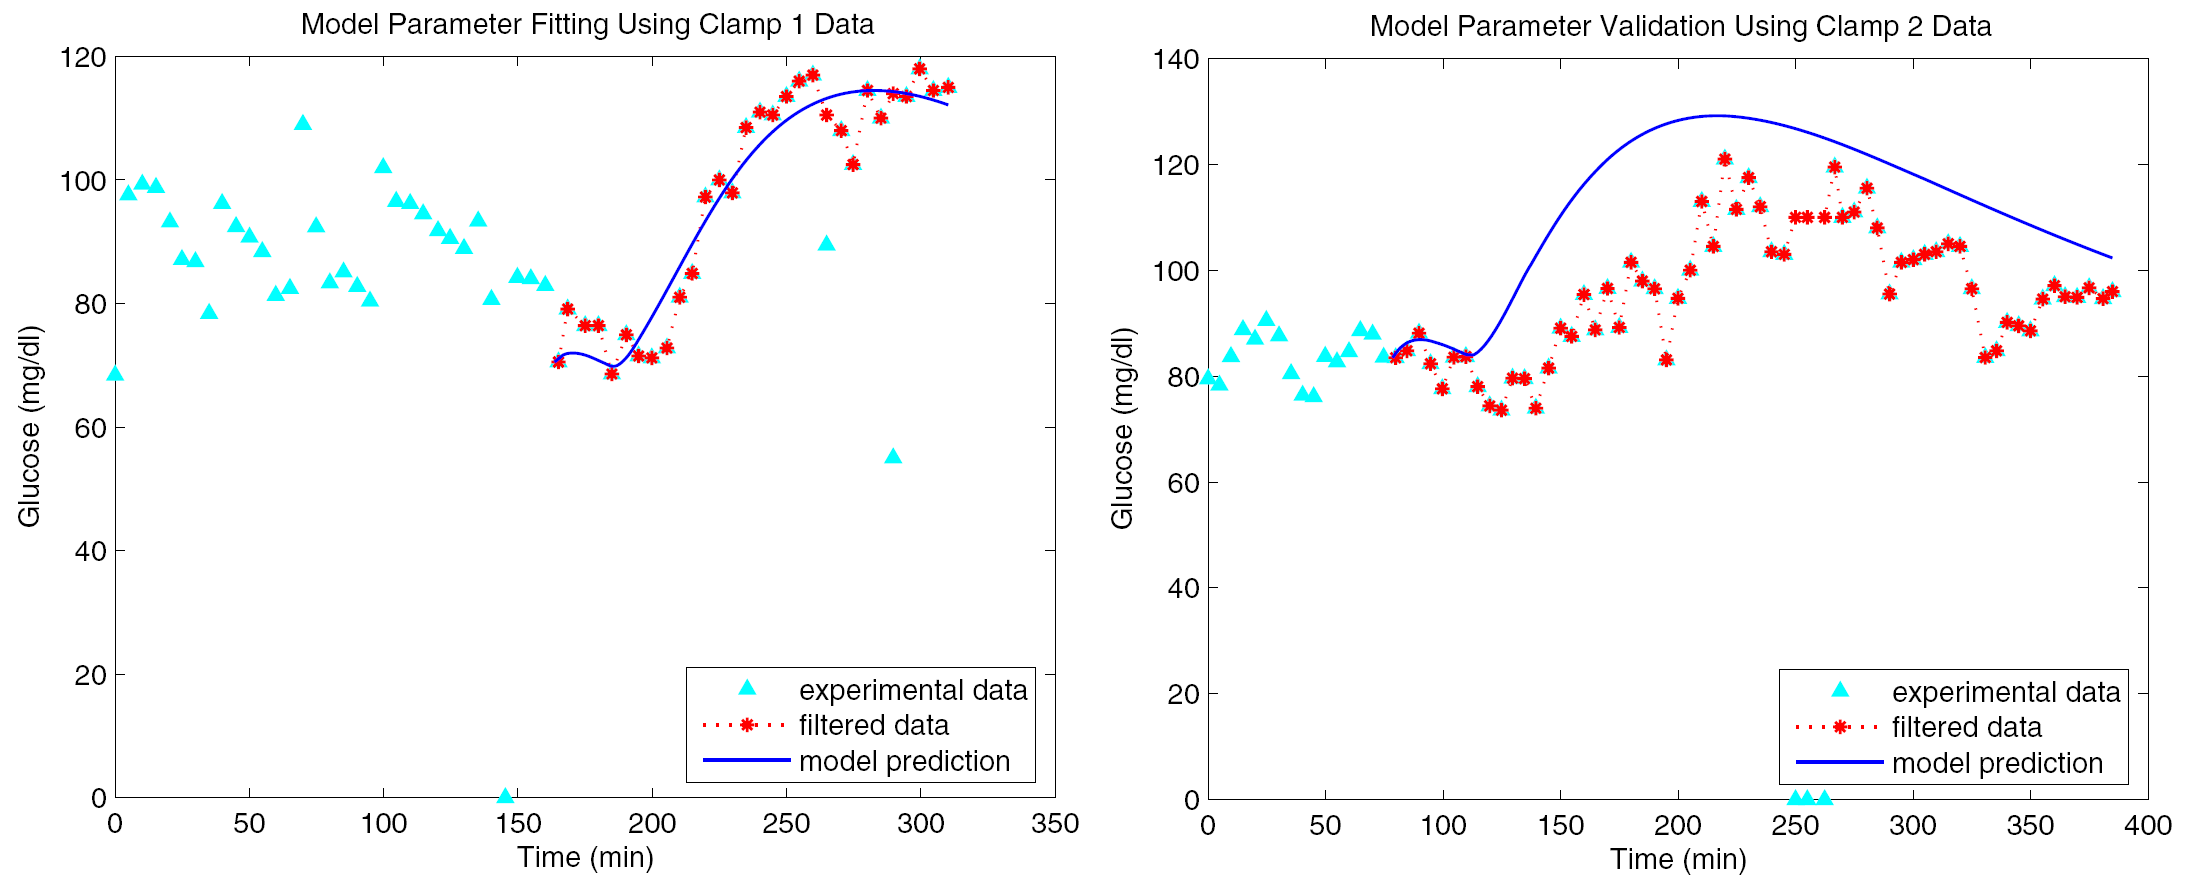
\epsfig{file=Figures/palerm_identification_composed.png, width=\textwidth}\caption{Model prediction versus data for one of the patients. Left graph shows the fitting of the data. Right graph shows the validation data on the same patient.}
%\label{fig:palerm_compare}
%\end{figure}

The work performed by Palerm \textit{et al.} supposed a solid first approach to the identification problem, but still, unsuccessful. The predictions were not able to mimic the response of the patients in different days, which can be caused either by model mismatch to the actual physiology or variations in the parameters within the same patient, or even maybe the incorrect use of data for identification.

Finan \textit{et al.} proposed a comparison of models identification for diabetic patients based on ARX models \cite{finan2009experimental}. They used data from 9 type 1 diabetic patients for identification comparing every prediction to that of a Zero Order Holder (ZOH). The ZOH predictions consisted simply in maintaining the glucose level for as long a the prediction horizon is. The predictions of the models were tested for prediction horizons of 30, 60 and 90 minutes. The study concluded that non significant improvement on the prediction capabilities (Relative Mean Square Error of the validation days) was observed from using ARX models instead of a ZOH. This conclusion is of great importance for identification in type 1 diabetic patients, since it discourages the use of pure data-based models in the prediction of glucose concentration. The authors conclude that non-modeled disturbances hinder greatly the performance of the selected models, and that getting reliable quantitative measures of exercise and stress levels would result in better quality predictions.
%Van heusden comparison \cite{van2011control}

Concerning the lack of identifiability showed so far by all of the available models in literature, Simone del Favero \textit{et al.} approached the identification problem from a completely new angle \cite{del2012glucose}. They proposed a method for identification using clinical index instead of purely mathematical quadratic indexes for data fitting. The clinical index consisted in a weighted index based on the glucose prediction danger to the patient. The reasoning behind this kind of fitting is that predictions for clinical patients are not worse as they differ from actual data, but as they unable to detect situations in which the patient may be endangered. For example in the case where a patient is heading towards hypoglycemia and the predictions are those of high glycaemic levels.

\section{Experiment Design for Artificial Pancreas}
\label{sec:ExperimentDesign}

Model identification is limited by both the model complexity and the amount and quality of the available data. The current state of models for identification has already been stated. In this chapter we will focus on the improvement of data acquisition techniques in the diabetes environment.

Predictions of the identified models are highly dependent on the identifiability of the model itself. Identifiability of a model is the facility to repeat an identification of its parameters under similar circumstances. Identifiability of a model is mainly dependent on the models structure, but it can also be improved by performing experiments that ease the process of the identification. The process of preparing data gathering experiments in order to enhance the identifiability of the model is called Optimal Experiment Design. Optimal Experiment Design is rare on the diabetes context due to the fact that data acquisition usually occurs in a clinical environment, where there are physical and ethical limitations to the experimental conditions.

There is a set of clinical tests that can help clinicians to either diagnose diabetes or to identify clinical parameters of glucose homeostasis:

\begin{itemize}
	\item \emph{Oral Glucose Tolerance Test (OGTT).} This standard test is used for diagnostics of diabetes. The test starts in the morning with the patient following the usual physical activity as in a normal day. The previous evening a meal of 30-50 g of carbohydrates is consumed. In the morning, a fasting blood sample is collected and then a solution of 75 g of glucose in water is drunk over a period of 5 minutes. Blood is then monitored afterwards at intervals. The most common interval though is a single sample (plus the fasting sample) 2 hours after the glucose solution ingest.
	\item \emph{Intravenous Glucose Tolerance Test (IVGTT).} This standard test is used for measuring the pancreas activity either in a healthy person or a diabetic patient. The glucose is administered in a antecubital vein over 60 seconds using a dose of 300 mg/kg. Glucose (and potentially insulin) is monitored starting at the moment of the infusion, with a fast sampling period (5 minutes or less) in the first period of the experiment, and more distanced measured at the end, lasting the whole of the experiment at least 3 hours.
	\item \emph{Postprandial Glucose Test.} This test is used to screen for diabetes and to evaluate treatments of therapies in diabetic subjects. The patient eats a balanced meal of measured components with a carbohydrate content of 100 g or more. The patient is then monitored for a minimum of two hours, and in case of necessity of testing a therapy, it is applied normally to the patient. This test is the easiest to perform since it follows the daily routine of the patients with a tight monitoring of blood glucose.
	\item \emph{Clamp Glucose Test.} Clamp tests are a battery of experiments that consist in artificially keeping blood glucose levels steady by intravenously infusing either glucose solution and/or insulin. They are difficult to perform as they require of an skilled doctor adjusting the glucose infusion levels to the appropriate concentration in order to lead blood glucose to the desired range. An example of clamp test is the euglycaemic hyperinsulinemic clamp, which consists on administering a large insulin infusion while maintaining glycemia in a controlled range of 90-100 mg/dL. This test permits the quantification of the insulin resistance of the patient without risking the patient to go to hypoglycemia.
\end{itemize}

Much more complex experiments can be performed for measuring metabolic fluxes in diabetic patients, as for example methods with radioactive tracers can help in the characterization of emptying rates in the digestive tract. In 2003 Basu \textit{et al.} described a triple-tracer method for assessing the postprandial glucose metabolism \cite{basu2003use}, which was later used by Dalla Man \textit{et al.} for developing a model of the gastrointestinal absorption of glucose \cite{man2007meal}. This type of tests though are extremely difficult to perform, even with single tracers; they require specialized instruments for the detection of the isotopes, and they are also much more intrusive to the patients involved

The field of optimal experiment design for diabetes has been developed greatly by Federico Galvanin and his team. In 2009 they published a design of a postprandial monitoring experiment with a variating insulin infusion throughout the post-prandial period \cite{galvanin2009}. The approach they used leads to results dependent on the model used, which for their case was the Cambridge model described earlier. They based their design on the optimality of 5 parameters of the endogenous glucose-insulin model, attempting to minimize the uncertainty in the identification of those parameters. After \textit{a priori} sensitivity analysis, they realized that two of the 5 parameters are highly correlated in the postprandial period and cannot be identified together so they reformulated the problem as the optimization of identifiability of 4 parameters, one of which was the ratio between the unidentifiable parameters. The outcome of the experiment design was a 2 meal monitoring where they tunned the CHO content of the meals and the insulin infusion from an insulin pump. The outcome of the experiment was relatively complex with the insulin infusion profile defined as a piecewise constant function with 12 levels and 11 level switching times.
%\begin{figure}[hbtp]
%\centering
%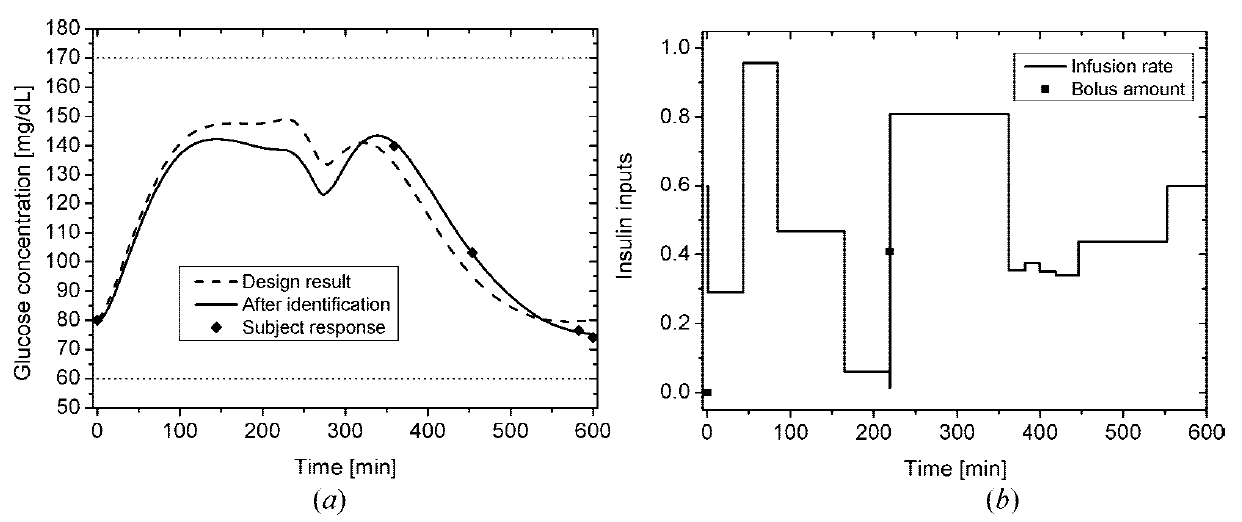
\epsfig{file=Figures/galvanininsulin.png, width=\textwidth}\caption{In the left panel the result of a simulation of the virtual patient is shown for the two meals period. In the right panel can be seen the piecewise function result of the experiment design for the insulin infusion.}
%\label{fig:galvanininsulin}
%\end{figure}

The qualitative result shown in the experiment design proposed by Galvanin \textit{et al.} is actually difficult to implement in a real experiment. Given that the models used are inaccurate, it is not advised to take the results of the experiment design accurately. Nevertheless, the results of this paper are very useful: it demonstrates that identifiability in diabetes is increased for longer experiments, and it shows that exciting the insulin input, statistically satisfactory parameter estimation can be achieved.

Later on, Galvanin \textit{et al.} published another work on optimal experiment design using on-line updates to the identifiability of the parameters \cite{galvanin2011optimal}. They realized from previous experimentation that model-based experiment design was too dependent on the model used. They decided to approach the issue in this paper introducing a model mismatch, based on the simple idea of simulating the data with one literature physiological model (in this case de UVA model) and identifying with another (the Cambridge model). The experiment design outcome is very similar to that of the previous work, with step shifts on the insulin infusion to the patient. %The new design is depicted in Figure \ref{fig:galvaninombre}.
%\begin{figure}[hbtp]
%\centering
%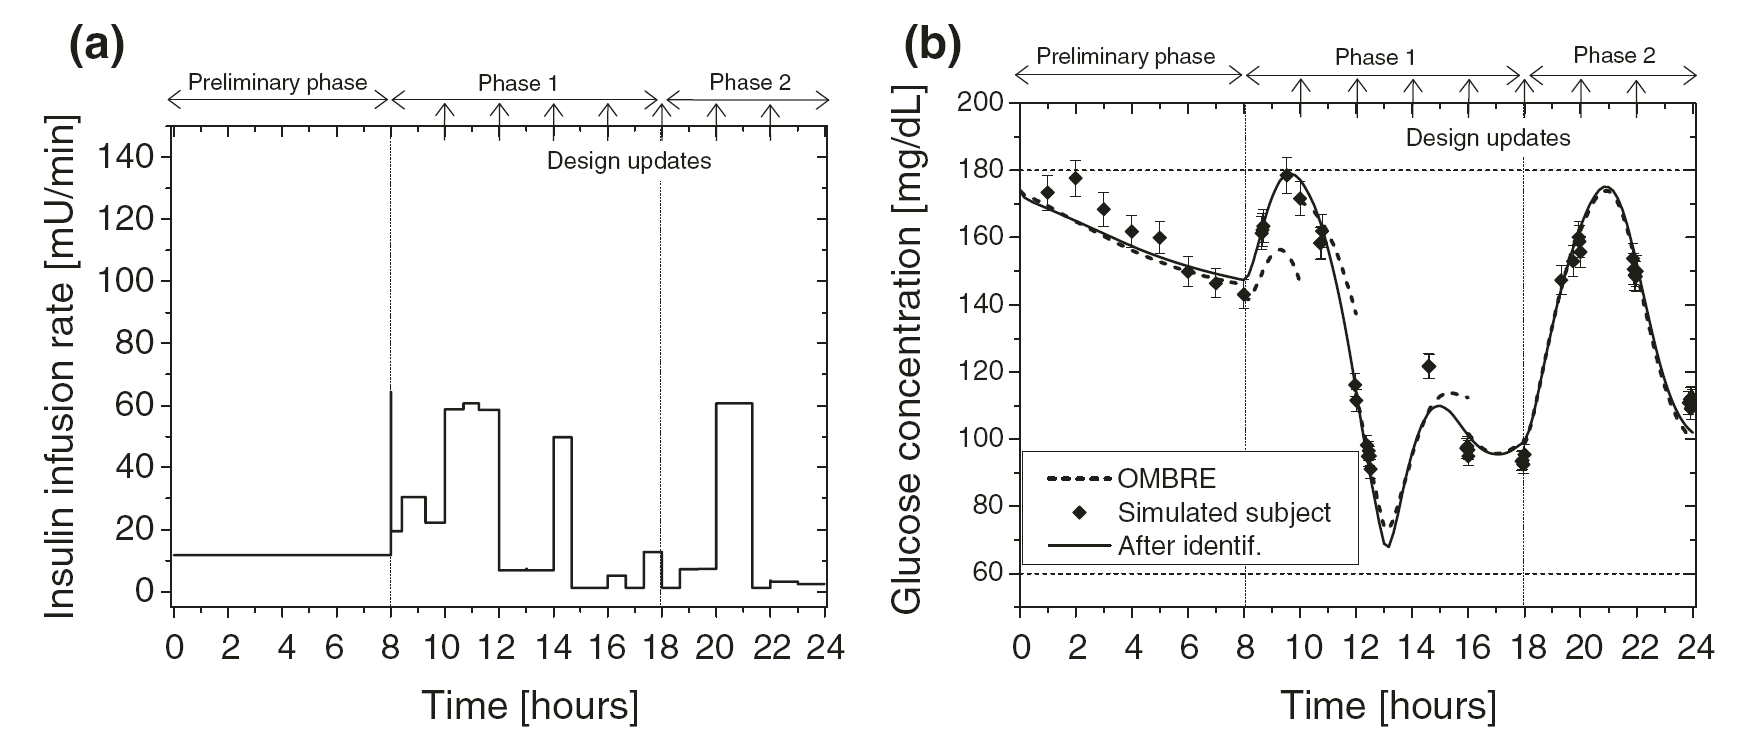
\epsfig{file=Figures/galvaninombre.png, width=\textwidth}\caption{In the (a) panel the insulin infusion is shown for the whole duration of the experiment. In the right panel the blood glucose concentration of the patient is displayed, including the identified model's predictions and simulations.}
%\label{fig:galvaninombre}
%\end{figure}

Galvanin \textit{et al.} concluded the study with a feasibility analysis of the experiments designed. When introducing the model mismatch, the classic model based experiment design was unable to provide feasible experiments. When using the on-line experiment redesign and identification, feasibility was achieved, and identifiability of the parameters was greatly improved. However, the amount of glucose and insulin to be delivered with the new method was much more aggressive. Clearly, this is unfeasible and unethical in the clinical setting as it would pose patients safety at risk.

Cobelli and Thomaseth published a study of optimal inputs for the Bergman minimal model using also optimality of identification of the parameters of the model \cite{cobelli1987minimal}. They focus on the design on finding optimal continuous functions of excitement to the endogenous model. They concluded that the outcomes of the experiment are very interesting from the modeling point of view, but of limited relevance in the diabetes context. Indeed, the optimal inputs obtained are too difficult to realize in clinical practice. They also imply that delayed insulin inputs can be useful for identification of certain parameters of the model.

Few other relevant works on the field of experiment design have been published. However, modifications on the traditional inputs with the aim of improving data quality is often seen in research of the artificial pancreas. Percival \textit{et al.} for example used delayed insulin bolus (2 hours after the meal) for the data acquisition of glucose profiles for a control algorithm \cite{percival}. %The scheme for the experiment monitoring and inputs can be seen in Figure \ref{fig:percival}
%\begin{figure}[hbtp]
%\centering
%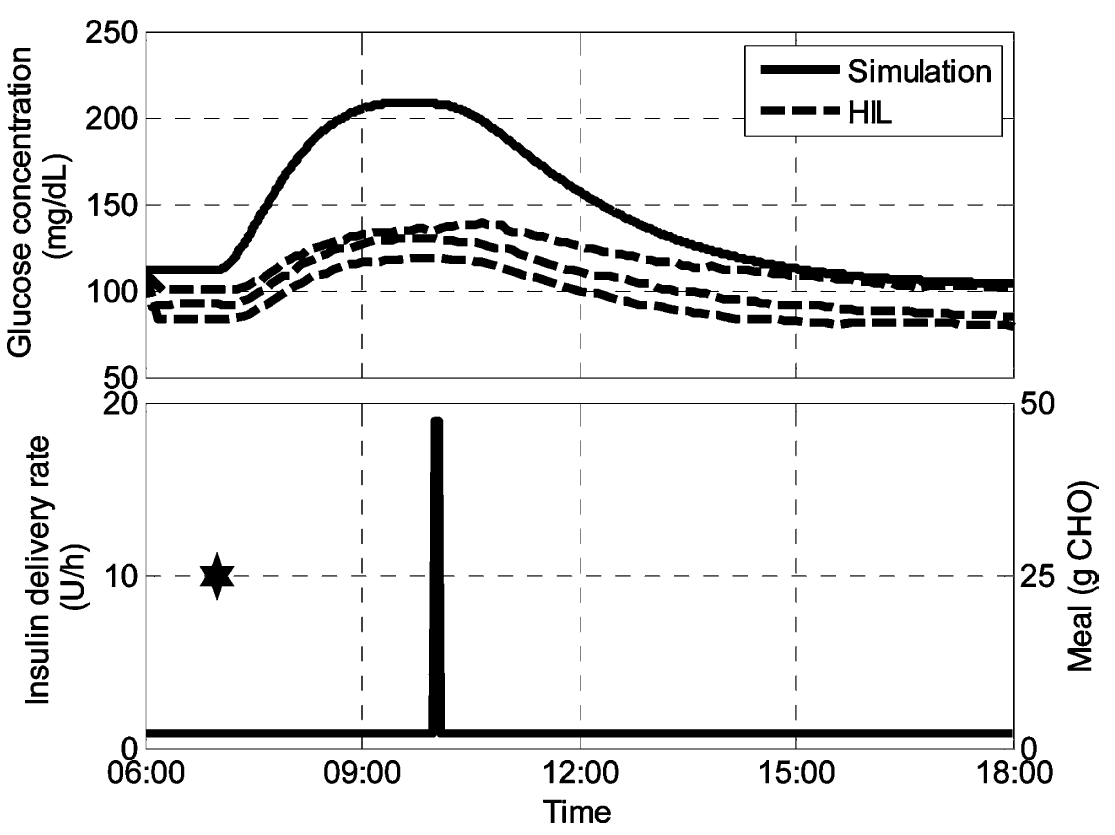
\epsfig{file=Figures/percivalshift.png, width=0.7\textwidth}\caption{Top panel shows the glucose simulation and CGM estimations for several calibration methods. Bottom panel corresponds to the inputs of the system for the same period. The star points at the meal ingestion time, and the impulse is the insulin bolus time.}
%\label{fig:percival}
%\end{figure}

Even though the clear objective of Percival \textit{et al.} when shifting the bolus time was to enhance the identifiability of the model, there is no further justification to it. In general, diabetes research lacks on simple experiments designed for the day-by-day routine of the diabetic patient; simple and safe enough experiments that will imply the patient participation and understanding of the disease he is living with, and the research related to it.

\section{Uncertainty and Interval Identification in Diabetes}
\label{sec:IntervalIdentificationInDiabetes}

Individualization of models for diabetes is greatly hindered by the fact that few models in literature consider intra-patient variability. In the models described in Section \ref{sec:ModelsForDiabetes} every model parameter stands for a physiological constant or function, and it is assumed to be characteristic to each patient. Most of the model proposed are published with some distribution in their parameters that resemble population values. These population values are an accepted quantification of the inter-patient variability for the parameters evaluated. However, characterization of a patient is dependent on the current metabolism of the patient, which is highly variable. This intra-patient variability has been regarded in literature with little detail.

One of the main sources of metabolic variability is the circadian rhythm of the patient. It is well established that the circadian variations of diabetic patients cause above average glucose levels in the early morning (event known as ``Dawn Phenomenon''), among other effects. The circadian effect has been quantified in the insulin dependance by Scheiner and Boyer \cite{scheiner2005characteristics}, showing a higher insulin relative dosage needed in the morning in type 1 diabetic patients. Higher insulin demand combined with constant basal infusion rates directly results in high morning glycemia, such as the reported in the Dawn Phenomenon. This work shows how insulin basal rate decreases for every age group after breakfast time, showing a periodic behavior of one of the better known physiologic parameters in diabetes: the insulin sensitivity. Furthermore, this work emphasizes the great difference in the population values when distributed by age groups, and suggests that a single probability distribution is not sufficient to characterize one parameter for the type 1 diabetic population.
%\begin{figure}[hbtp]
%\centering
%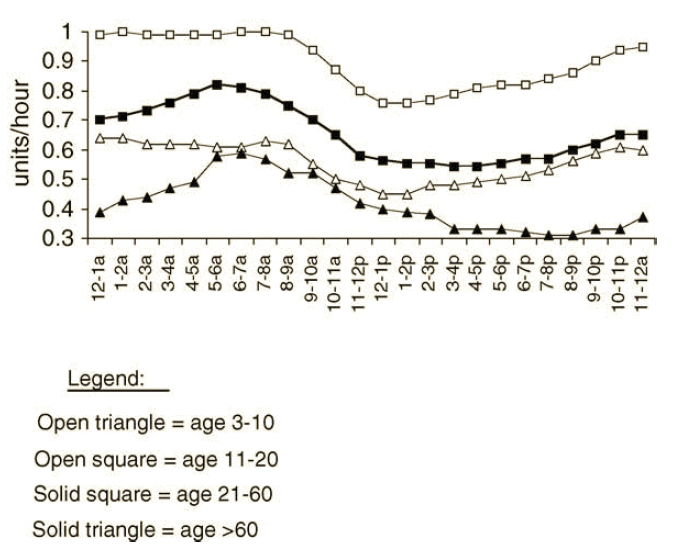
\epsfig{file=Figures/scheinercircadian.png, width=0.8\textwidth}\caption{Average hourly basal rate values by age group.}
%\label{fig:scheiner}
%\end{figure}

Understanding that physiologic parameters are not correctly characterized by only a number, several authors in recent years have been adapting physiological models in order to simulate patients with variability inherently considered. Using interval analysis methods and models is a new way of considering those parameters. Interval models consider internal parameters as ``ranges'' instead of punctual numbers. The parameter at a given time is actually unknown, but it is known to be comprised within the boundaries of the interval that defines it. The outputs of interval models are also intervals, and in the case of diabetes, the main output being glucose, means that we have to work with uncertain ranges of glucose.

Calm \textit{et al.} published work based on the Cambridge where modal interval analysis is applied for the plasma glucose prediction to face uncertain food intake and patient parameters such as insulin hepatic and peripheral sensitivity \cite{calm2007prediction}. The model was later validated against Monte Carlo simulations proving it to be a much more efficient in computation \cite{calm2010comparison}. The interval model developed was tested against several scenarios where parameters in the insulin absorption and meal absorption models were considered to have between a 10\% and 20\% variation. In general, wider variability considered in the parameters yield wider glucose outcomes. Calm \textit{et al.} showed that even relatively small variations considered in the parameters of the model (10\%) yield wide glucose prediction bands (approximately 100 mg/dL). Considering that sensitivity parameters of a real diabetic patient can be much more variable than the 10\% considered by this study, even larger glucose prediction bands are expected when characterizing diabetic patients in an experimental setting.
%\begin{figure}[ht]
%\centering
%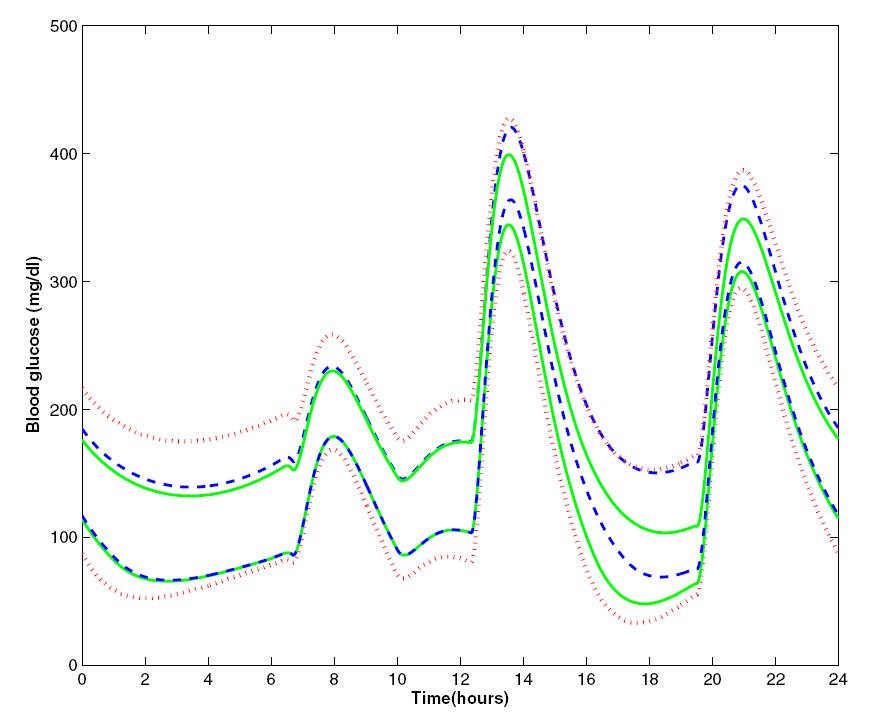
\epsfig{file=Figures/calmhovorka.png, width=0.9\textwidth}\caption{Envelopes obtained with the interval model for three different scenarios: 10\% variation in insulin sensitivity parameters (solid line), 20\% variation in insulin sensitivity parameters (dotted line) and 10\% variation with modified insulin bolus (dashed line).}
%\label{fig:calmhovorka}
%\end{figure}

Another approach to interval models simulation was undertaken by de Pereda \textit{et al.} on the Cambridge model \cite{de2012prediction}. They tackled the uncertainty analysis by using monotonicity analysis of the states of the model and its critical points. The bounds provided by this type of analysis are very similar to those proposed by Calm \textit{et al.}, but with the advantage of considering more parameters subject to uncertainty, as for example the insulin absorption lag time $t_{maxI}$. They also proposed the use of the uncertainty model as a short-term prediction tool, showing that for smaller prediction horizon scenarios, band widths do not grow excessively, and are suitable to use in regulation algorithms such as Model Predictive Control. The work done by de Pereda \textit{et al.} is very recent (2012), and it still has to be tested as a suitable method for identification and control.

To our knowledge, Kirchsteiger \textit{et al.} published the only identification procedure with consideration of uncertainty so far \cite{kirchsteiger2011estimating}. This work was initially based on a simple data-based transfer function model with 6 interval parameters. The identification was performed on data from 9 patients and three postprandial periods for each patient. After some trials, a simplified model structure was proposed for identification, due to identifiability issues, reducing it to only 4 interval parameters. The identification was posed as an optimization problem, where not only the fitting error was identified for 3 days, but also the standard deviation of each parameter considering the three postprandial periods. This procedure kept the parameters from resulting in too wide intervals, while still fitting the data of the patient. Even though the idea of identification of 3 separate days with common parameters is appealing, the study lacked of the proof of cross-validation on the data. Validation on single meals was performed, but not using the interval parameters, neither selecting a day \textit{a priori} as the validation day. It is unclear whether the day used for validation was just the 3rd day chronologically or the best case validation. Also, the data source on this study was treated without consideration of the possible errors introduced, which is a very important issue if not using glucose reference data.
%\begin{figure}[hbt]
%\centering
%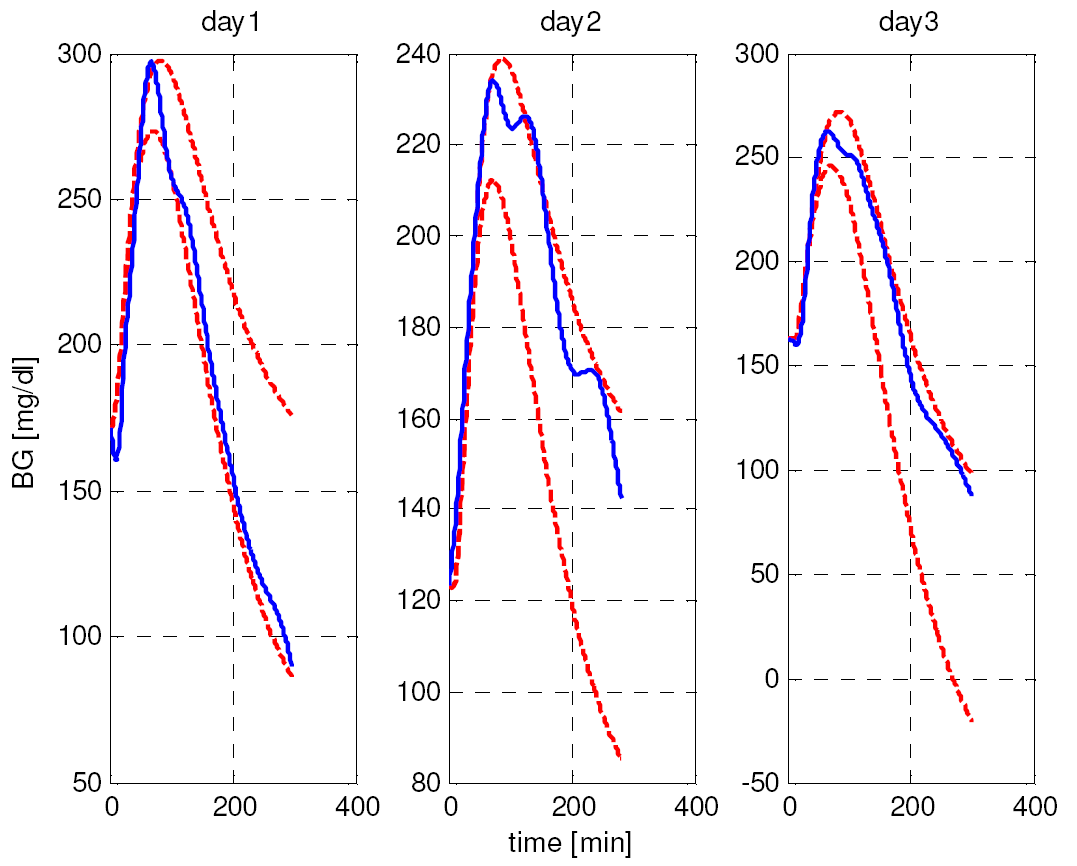
\epsfig{file=Figures/kirchsteiger.png, width=0.8\textwidth}\caption{Three-day identification of a diabetic patient's breakfasts. Blue solid line represents the spline-interpolated experimental glucose measurements. Red dashed lines are the upper and lower bounds given by the model.}
%\label{fig:kirchstegier}
%\end{figure}



